\documentclass{standalone}
\usepackage{graphicx}	
\usepackage{amssymb, amsmath, amsthm}
\usepackage{color}

\usepackage{tikz}
\usetikzlibrary{intersections, backgrounds}

\definecolor{light}{RGB}{220, 188, 188}
\definecolor{mid}{RGB}{185, 124, 124}
\definecolor{dark}{RGB}{143, 39, 39}
\definecolor{highlight}{RGB}{180, 31, 180}
\definecolor{gray10}{gray}{0.1}
\definecolor{gray20}{gray}{0.2}
\definecolor{gray30}{gray}{0.3}
\definecolor{gray40}{gray}{0.4}
\definecolor{gray60}{gray}{0.6}
\definecolor{gray70}{gray}{0.7}
\definecolor{gray80}{gray}{0.8}
\definecolor{gray90}{gray}{0.9}
\definecolor{gray60}{gray}{0.95}

\begin{document}

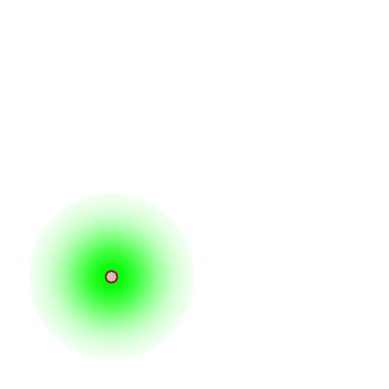
\begin{tikzpicture}[scale=0.35, thick]
  \draw[white] (-4, -4) rectangle (8, 8);
 
  \foreach \i in {1, 0.99, ..., 0} {
    \pgfmathsetmacro{\prop}{100 * exp(-3.0 * \i * \i)};
    \colorlet{custom}{green!\prop!white};
    \fill[custom] (-1, -1) circle ({3 * \i});
  }
  
  \fill[color=dark] (-1, -1) circle (7pt); 
  \fill[color=light] (-1, -1) circle (5pt);

\end{tikzpicture}

\end{document}  